\documentclass{article}
\usepackage[ruled,vlined,linesnumbered]{algorithm2e}
\usepackage{algpseudocode}
\usepackage{amsmath}
\usepackage{amsthm}
\usepackage{graphicx}
\usepackage{subfigure}
\usepackage{float}
\usepackage{amsmath }
\usepackage{amsfonts }
\usepackage{pdfpages}
\usepackage{epsfig}
\usepackage{graphicx}
\usepackage{arydshln}
\usepackage{verbatim}
\usepackage{subfigure}
\usepackage{enumerate}
\usepackage{rotating}
\usepackage{threeparttable}
\usepackage{caption}
\usepackage{epsfig}
\usepackage{cite}
\usepackage{geometry}
\geometry{a4paper, top=2.54cm, bottom=2.54cm, left=3.18cm, right=3.18cm}
\theoremstyle{definition}
\newtheorem{prob}{Problem}
\newtheorem{ans}{Answer}
\usepackage[colorlinks,linkcolor=black]{hyperref}
\linespread{1.2}
\begin{document}
	\title{Assignment 3}
	\author{Kailing Wang 521030910356}
	\date{November 10.2022}
	\maketitle
	\begin{prob}
		(25 points) You are given $n$ jobs, where each job $j$ has its processing time $p_{j}$ and weight $w_{j}$. We need to process all of them on one machine. We use $C_{j}$ to denote $j$ 's completion time in a schedule. Our goal is to find the best schedule that minimizes the average weighted completion time (i.e., $\min \frac{\sum_{j=1}^{n} w_{j} C_{j}}{n}$ ). Design a greedy algorithm for it.
	\end{prob}

	\begin{ans}
		~
		
		The weighted completion time distributed by a job is its weight multiplies the sum of time of the job and previous jobs. Considering this, we want jobs with larger weight done earlier. The simple way is simply finish the job with the largest weight first. Algorithm Job-Sort shows the pseudo-code. 
		
		\begin{algorithm}
			\caption{Job Sort}
			\KwData{$n$ jobs with processing time $p_j$ and weight $w_j$}
			\KwResult{The job finishing plan}
			\BlankLine
			Sort the jobs according to the average-weight\;
			\While{Not Done}
			{
				Do the jos with largest average-weight\;
			}
			It's done\;
		\end{algorithm}
	
		The average-weight is defined as $\frac{w_j}{p_j}$
			
		Time complexity is the same as the sort: can be $O(n\log n)$. To prove time complexity, we only need to prove if we change a job with larger weight in the front with another job with less weight behind. 
		
		Suppose we have $(p1,w1,C1)$ and $(p2,w2,C2)$. Here $\frac{w1}{p1}>\frac{w2}{p2} \text{ and } C1<C2$, and the total job weight between them is $w$. Then we change the to job in position. We only need to calculate the total change of weighted completion time. The moved back job contributed $w1\cdot C2-w1\cdot C1$ change. The moved forward job contributed $w2\cdot (C1-p1+p2)-w2\cdot C2$. The jobs between contributed $w\cdot (C2-p1)-w\cdot (C2-p2)=w\cdot (p2-p1)$. The total change is 
		$$(w_1-w_2)\cdot (C_2-C_1)+(w+w_2)\cdot p_2-(w+w_2)\cdot p_1$$
		Note that $C_2-C_1\geq p_2$, and so 
		$$
		\begin{aligned}
			(w_1-w_2)\cdot (C_2-C_1)+(w+w_2)\cdot p_2-(w+w_2)\cdot p_1 \\ \geq (w_1-w_2)\cdot p_2+(w+w_2)\cdot p_2-(w+w_2)\cdot p_1 \\ =(w+w_1)\cdot p_2-(w+w_2)\cdot p_1
		\end{aligned}$$
		, from $\frac{w1}{p1}>\frac{w2}{p2}$ we have $\frac{w+w1}{p1}>\frac{w+w2}{p2}$. $(w+w_1)\cdot p_2-(w+w_2)\cdot p_1\geq 0$, the change is always positive. This proves the correctness.
		\end{ans}

	\begin{prob}
		(20 points) You are given $n$ prices $p_{1}, p_{2}, \cdots, p_{n}$, where $p_{i}$ represents the $i$-th day price of a stock. On the $i$-th day, you are allowed to do one of the following operations:
	
	\begin{itemize}
	\item Buy one unit of stock and pay $p_{i}$. Your stock will increase by one.
	
	\item Sell one unit of stock and get $p_{i}$ if your stock is at least one. Your stock will decrease by one.
	
	\item Do nothing.
	
	\end{itemize}
	
	How to maximize the profit (the money left after $n$ days)?
	
	Professor Tao thinks the question is easy and designs the following greedy algorithm: We enumerate from day 1 to $n$ and maintain a min-heap. In each iteration, we do two operations:
	
	\begin{enumerate}
	\item We insert $p_{i}$ into the heap.
	
	\item Let $q$ be the minimized price in the heap. If $q<p_{i}$, we increase profit by $p_{i}-q$, pop $q$ from the heap, and insert $p_{i}$ into the heap.
	
	\end{enumerate}
	
	Finally, Professor Tao claims profit is the maximized profit we can get. Do you think Professor Tao is correct? If yes, prove the correctness. Otherwise, give a counterexample. 
	
	\end{prob}

	\begin{ans}
		~
		
		Professor Tao is correct. To explain the correctness, first assume in the $k-1$ day, we've got the best policy using Tao's algorithm. Obviously for the first day it is correct: there's no profit to make. Now let's check the situation on the $kth$ day. 
		
		The price on the $kth$ day is $p_k$. We should adjust the policy to make better profit on the base of the previous policy. For now forget about the algorithm. If we want the profit to increase, we only have to consider buying a stock cheaper than $p_k$ and selling it today. Check all the $p_i<p_k$, for each $p_i$,  discuss as follows:
	
		\begin{enumerate}[(a)]
			\item We can't find any price smaller than $p_k$, like plot (a). The best profit is the same as the one for last day. 
			\item We find $p_i$ smaller than $p_k$ and $p_i$ was not bought before(we don't mind if we sold stock on this day, because if we do buy and sell at the same time, we actually do nothing), like plot (b). We can try to buy the stock on day $i$. This case, we get $p_k-p_i$ more profit. 
			\item We find $p_i$ smaller than $p_k$ but sold at $p_j$ larger than $p_k$, like plot (c). For this case, however we change the policy, we can't make more profit. The profit is still the same. 
			\item We find $p_i$ smaller than $p_k$ and sold at $p_j$ smaller than $p_k$, like plot (d). This case, we should change the policy by changing the selling time point from $k\text{ to }i$. However, there may exists $p_m$ that is smaller than $p_j$ and satisfies case (b), like plot (e). We have to solve this problem recursively: adjust the policy before day $j$. 
		\end{enumerate}
	
		\begin{figure}
			\centering
			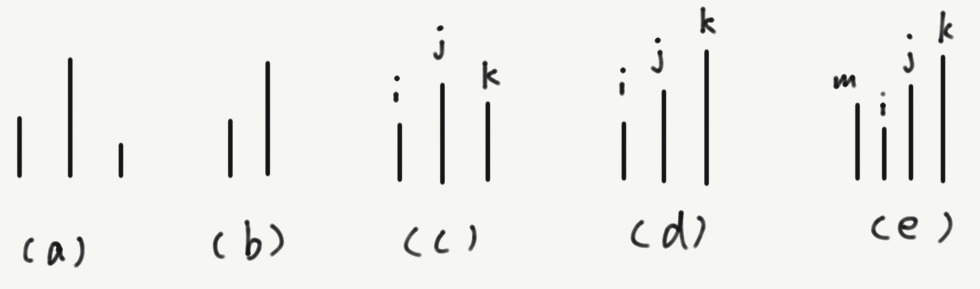
\includegraphics[width=0.7\linewidth]{plot}
			\caption{Plots}
			\label{fig:plot}
		\end{figure}
		
		First I'll also explain why when we pop a head, we push the new p into heap again: the first pop of this new p means we do nothing this day, and the second time it is popped means we buy stock on this day. And since we pop when we buy, the prices in heap are all on days we are allowed to buy stock. Another thing to explain is that if we want to replace a sell date, we can simply buy stock on the date to be replaced. The profit change is the same.
		
		We have to prove that from the best profit policy in $k-1$ days, using Tao's algorithm we can obtain the best policy for all $k$ days. In the unknown new policy, discuss the situation with day $k$: We may do nothing(if only case (a) and (c) happens) or buy one more stock and sell it(if case (b) and (d) exist). 
		
		If the best policy is do nothing, it's naive. According to Tao's algorithm, the $p_i$ is not in the heap, and so the $p_k$ smallest now and is the new head of the heap. The profit remains the same. We can obtain the best policy this way.
		
		If in the best policy we buy stock like case (b) and sell on the $kth$ day, the best profit is the sum of the previous best profit and the added profit. The added profit is fixed, and if we want to obtain max profit in the previous $k-1$ days, we still use the old policy. Using Tao's algorithm, we simply find a smallest price on days we are allowed to buy stock. So we can also obtain the best policy. 
		
		If the best policy is we buy stock like case (d). Let's say Tao's algorithm sells the stock bought on day $m$. However, the best policy sells the stock bought on day $n$, and gets more profit than Tao. On the previous days, the best policy is different from the policy given by Tao's algorithm. Can this happen? First, if this happens, the best policy earns $p_k-p_n$ on the last day while Tao earns $p_k-p_m$. Since we assume the best policy earns more but does not take the Tao's algorithm on $k-1$ days(we have assumed Tao can get the best profit on $k-1$ days), we have $p_n<p_m$ and the best policy earns at least $profit_{Tao's}-(p_m-p_n)$. Since in the best profit $n$ is the buy-in date, we can simply ignore it and continue. The best profit we can achieve with the rest $k-2$ days is to use Tao's method. In Tao's policy on $k-1$ days, $n$ must be a buy-in date because $p_n<p_m$. Compare Tao's policy on $k-1$ days and the $k-2$ days(without $n$), the difference can only be either we find a day $t$ after $n$ to buy the stock, like plot (f), or we don't buy this stock plot (g). In both cases we lose more than $p_m-p_n$ money: contradiction. In conclusion, the best policy can't be better than Tao's method.
		
		\begin{figure}
			\centering
			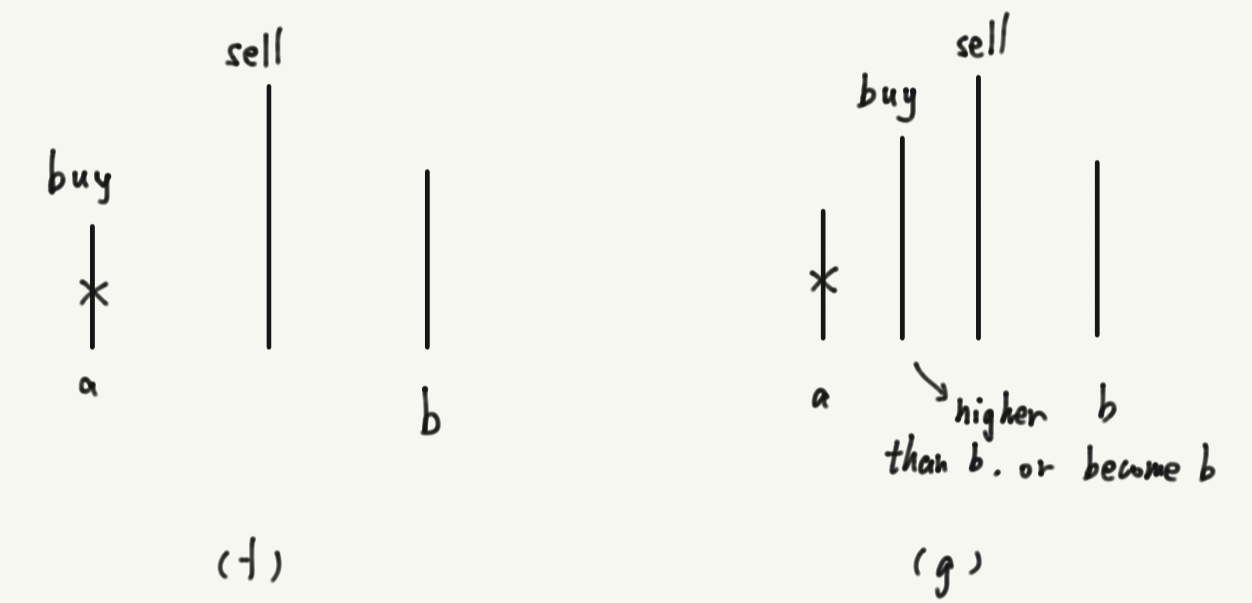
\includegraphics[width=0.55\linewidth]{../Assignment3tex/plot2}
			\caption{More Plots}
			\label{fig:plot2}
		\end{figure}
	
		Finally we can say Tao is correct. 
	\end{ans}
	
	\begin{prob}
	(30 points) There are $n$ players who need cakes, whose requests are $x_{1}, x_{2}, \cdots, x_{n}$. You are asked to buy one piece of cake and then cut it to satisfy everyone's request. However, The "cut" operation is lossy. Whenever you make a "cut" operation to size $W$ cake, you will lose the $p$ fraction of the cake. (E.g., if you cut a cake at the median with size 2 and $p=0.5$, you will get two pieces of cake with size $0.5$, and the loss is 1 . When you cut the $0.5$ size cake again, you will lose $0.25$ again.)
	
	(a) (5 points) There are four players where $x_{1}=x_{2}=x_{3}=x_{4}=1$, and $p=0.5$. what is the minimum size? Write down how you cut the cake. You don't need to prove it.
	
	(b) (5 points) There are four players where $x_{1}=x_{2}=1, x_{3}=x_{4}=3$, and $p=0.5$. What is the minimum size? Write down how you cut the cake. You don't need to prove it.
	
	(c) (20 points) Given $n$ players, their requests, and the loss factor $p$, design an efficient algorithm to find the minimum size of cake you need to buy.

	\end{prob}

	\begin{ans}
		~
		
		\begin{enumerate}[(a)]
			\item I need cake with size 16. I'll cut the cake by half and the cake become two 4 pieces, and then cut each piece by half and get four 1. Another way is to cut for 1s one by one, but will cost 22.
			\item I need cake with size 32. Cut it into 8-8, and cut each 8 into 1-3. Or cut into 12-4 and then 3-3, 1-1.
			\item The problem is very like a Huffman code problem. So use Huffman code to generate a cake. Algorithm Cake-Generator shows how to generate smallest cakes from pieces, and the cut plan is the opposite of the generation.
			
			\begin{algorithm}
				\caption{Cake Generator}
				\KwData{num of players $n$ and their desires $x_i$, lose fraction $p$}
				\KwResult{The smallest cake size $W$}
				\BlankLine
				Put all the desired cake pieces with size $x_i$ into the cake generator\;
				\While{More than one pieces of cake in the generator}
				{
					Find the smallest two pieces\;
					Combine them into one piece with size $x_t$\;
					Resize the cake into $\frac{x_t}{1-p}$ and put it back to the generator\;
				}
				The remaining cake has the smallest required size\;
			\end{algorithm}
		
			The merge process will happen $n-1$ times, so the time bottleneck tend to be in the select smallest. Use a heap to do so. Here whether to use Fibonacci heap is the same. The heap construction is $O(n\log n)$, and there are $n-1$ times of 2 $\cdot popmin$ and $push$ operation. The overall time complexity is still $O(n\log n)$. In class we used two linked lists, but it doesn't improve much.
			
			The cake generator construct a binary tree with cake size as nodes. The Huffman tree calculate the value of leaf nodes by depth dots weights, and here we calculate weight by $2^{depth}$ dots weights. So the proof of correctness is the same.
			
			Suppose we are in partial-OPT. Then we merged two nodes that are not the smallest two. Change one of the smallest node with one merged node. we find the total cost smaller. Change another pair, and the cost is again smaller. Then we know so constructed tree is the smallest. 
		\end{enumerate}
	\end{ans}
	
	\begin{prob}
		(25 points) You are given a fractional number $p / q$, where $p$ and $q$ are two positive integers and $p<q$. Can you design a greedy algorithm to decompose it into the following form: $p / q=1 / a_{1}+1 / a_{2}+\cdots+1 / a_{k}$, where $a_{1}<a_{2}<a_{3}<\cdots<a_{k}$ are all positive integers? (For example, $2 / 3=1 / 2+1 / 6$ and $2 / 3=1 / 2+1 / 7+1 / 42$ are both valid decomposition, while $2 / 3=1 / 3+1 / 3$ is not.) Remember to analyze the time complexity. Your algorithm should at least terminate for every input. Notice that if you succeed, you prove the decomposition always exists for all fractional numbers.
	\end{prob}
	
	\begin{ans}
		~
		
		The simple greedy is just split a fraction as large as possible each time. The detailed pseudo-code is attached as algorithm Get-Fraction.
		
		\begin{algorithm}
			\caption{Get Fraction}
			\KwData{A fraction number $x=\frac{p}{q}$}
			\KwResult{A fraction sequence with different denumerator and 1 as numerator}
			\BlankLine
			\While{the numerator of x is not 1}
			{
				$x\gets x-\frac{1}{\lceil\frac{1}{x}\rceil}$\;
				Add $x$ to the answer sequence\;
			}
			It's over. That simple.
		\end{algorithm}
	
		There is another way to divide the $x$ into $p~\frac{1}{q}s$. For the second $\frac{1}{q}$, apply $\frac{1}{x}=\frac{1}{x+1}+\frac{1}{x\cdot(x+1)}$. Then for next $\frac{1}{q}$s, do this recursively. This amazing algorithm is correct and easy, but since the calculation time doubles each time, the time complexity is $O(2^p)$.
		
		To explain the time complexity of the better solution of mine, I need to first explain the correctness: let's call $\lceil\frac{1}{x}\rceil~a$. To calculate $a$ takes $O(1)$. Also we have $$x<\frac{1}{a-1}$$that is $$\frac{p}{q}<\frac{1}{a-1},~a\cdot p - q < p$$ Also the iteration process is $$x'=\frac{p}{q}-\frac{1}{a}=\frac{a\cdot p - q}{a\cdot q}\text{, the new numerator is less than }p$$ Then we can see the numerator decreases. Since the numerator is integer, it decreases at least 1 at a time. after $O(q)$ it will decrease to 1, and the iteration is over. So, the time complexity is $O(q)$.
		
		After some code simulation, the time expectation is far less than $O(q)$. For example, the fraction $\frac{415411}{1145141919810}$ stops after 5 iterations.
		
	\end{ans}
	
	\begin{prob}
		How long does it take you to finish the assignment (including thinking and discussing)? Give a score $(1,2,3,4,5)$ to the difficulty. Do you have any collaborators? Write down their names here.
	\end{prob}
	\begin{ans}
		~
		
		3 No. All especially p4 is original. 
	\end{ans}
\end{document}